\documentclass{article}
\textheight 23.5cm \textwidth 15.8cm
%\leftskip -1cm
\topmargin -1.5cm \oddsidemargin 0.3cm \evensidemargin -0.3cm
%\documentclass[final]{siamltex}

\usepackage{ctex}
\usepackage{verbatim}
\usepackage{fancyhdr}
\usepackage{graphicx}
\usepackage{amsmath}
\usepackage{amssymb}
\usepackage{float}
\usepackage{multirow}
\usepackage{colortbl}
\usepackage{amsthm}
\usepackage{bm}
\usepackage{tikz}

\textheight 23.5cm \textwidth 15.8cm
\topmargin -1.5cm \oddsidemargin 0.3cm \evensidemargin -0.3cm
\title{HW5 实验报告}
\author{PB20010429 侯相龙}

\begin{document}
\maketitle
\section{实验内容}
实现二维 As-Rigid-As-Possible 形状插值算法:

M. Alexa et al. As-Rigid-As-Possible Shape Interpolation. SIGGRAPH 2000


\section{实验原理}
\begin{itemize}
    \item 网格中的每个三角形初始的两条边$\vec{x_1}, \vec{x_2}$线性映射到终态$\vec{y_1}, \vec{y_2}$,设对应的2*2子矩阵为A
    \item 对A 做SVD 分解 $A = U\Sigma V^\text{T}$, 其中U和V为正交阵。
    
    对A继续分解,具体来讲 $A = XY$,其中
    \[X = UV^\text{T}, \quad Y = V\Sigma V^\text{T}\]
    \item 创建迭代式子(随时间):X(2*2的正交阵)有如下表示:
    \[
        \begin{bmatrix}
            \cos (\theta)  & \sin (\theta) \\
            -\sin (\theta)  & \cos (\theta)
        \end{bmatrix}
    \]
    假设迭代n次,那么每一次旋转角为$\frac{\theta}{n}$, 对应的矩阵
    \[
        \begin{bmatrix}
            \cos (\frac{\theta}{n})  & \sin (\frac{\theta}{n}) \\
            -\sin (\frac{\theta}{n})  & \cos (\frac{\theta}{n})
        \end{bmatrix}
    \]
    
    对于Y,它的矩阵直接使用更简单的插值:$Y = t*I+(1-t)*Y$ ,其中$t = \frac{i}{n}, i=1,2, \cdots,n$
    
    \item 再基于约束点的限制,可构造方程,用最小二乘法(求导)即得解。
\end{itemize}

\section{算法介绍与步骤}
\begin{itemize}
    \item 将输入的3D点转换成2D点,以便进行后续计算。

    \item 构建稀疏矩阵L
    
    \item 初始化变量b,用于存储计算得到的b向量。

    
    \item 设置最后一行的边界条件,即将最终点的坐标赋值给最后一行的b向量。
    
    \item 利用最小二乘方法求解线性方程组,得到形状插值的结果。
    
    \item 将插值结果转换回3D点,并返回结果
\end{itemize}



\section{测试数据与实验结果}
对大象网格(elephant\_s.obj,elephant\_t.obj)进行测试,实验结果如下

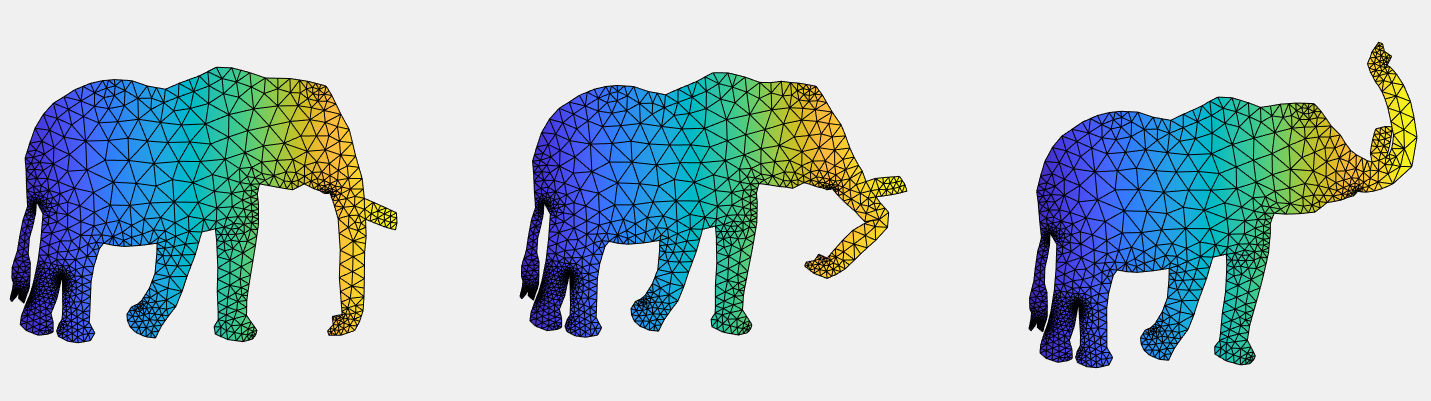
\includegraphics[width=0.7\linewidth]{0.png}

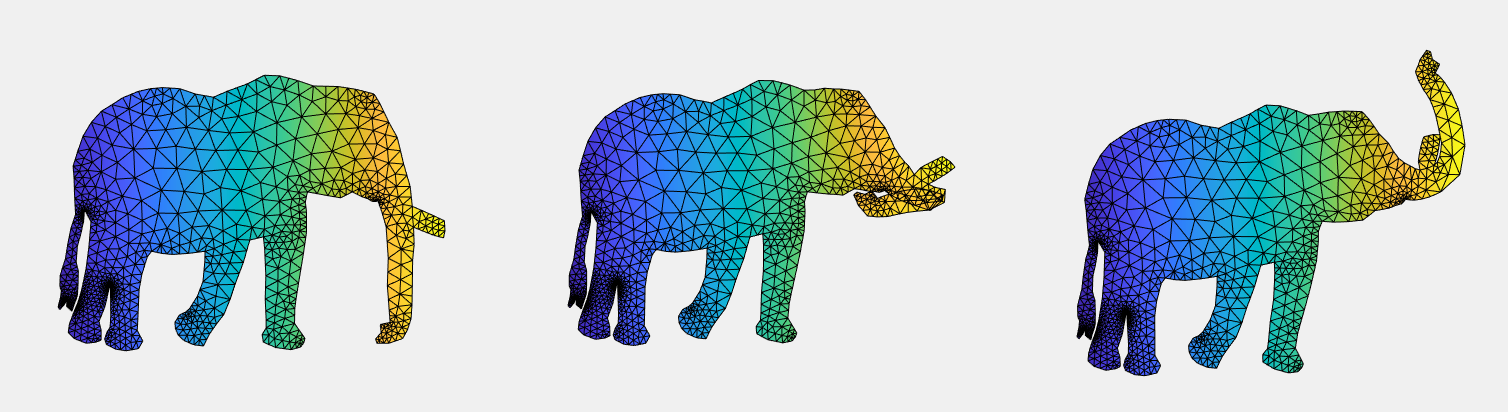
\includegraphics[width=0.7\linewidth]{1.png}

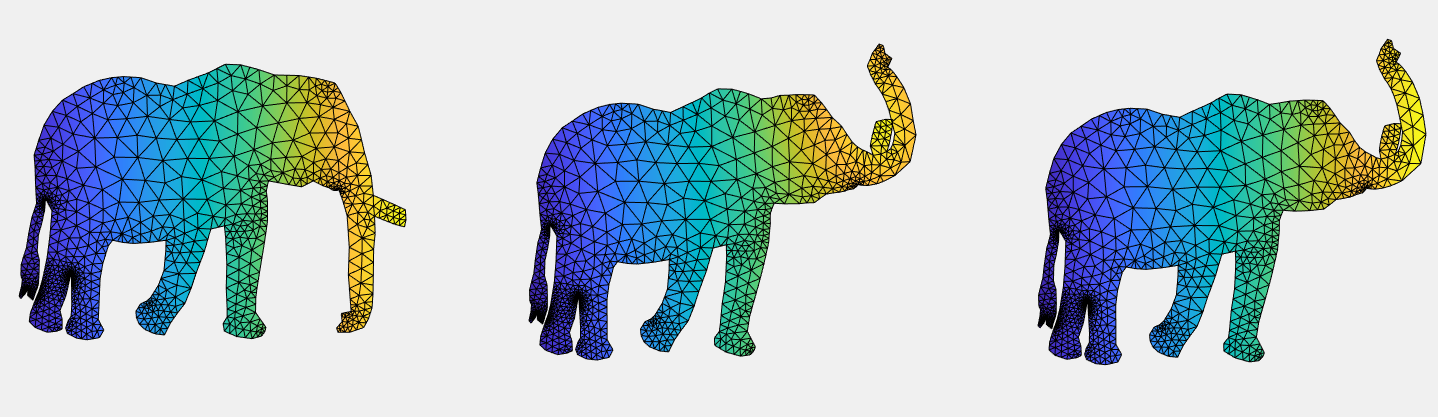
\includegraphics[width=0.7\linewidth]{2.png}




\end{document}
